% CSC 8851 Deep Learning, Fall 2026 -- Preliminary project report (CVPR 2026 author kit format).
% Build: pdflatex, bibtex, pdflatex, pdflatex. Needs cvpr.sty, ieeenat_fullname.bst, refs.bib and
% schema_figure.pdf in the same folder.
\documentclass[10pt,twocolumn,letterpaper]{article}
\usepackage[pagenumbers]{cvpr}

\usepackage{graphicx}
\usepackage{amsmath,amssymb}
\usepackage{booktabs}
\usepackage{multirow}
\usepackage{xcolor}
\definecolor{cvprblue}{rgb}{0.21,0.49,0.74}
\usepackage[pagebackref,breaklinks,colorlinks,allcolors=cvprblue]{hyperref}

\def\paperID{*****}
\def\confName{CVPR}
\def\confYear{2026}

\title{Query-Conditioned GNN Retrieval for Financial GraphRAG\\
{\large Preliminary Project Report, CSC 8851 Deep Learning, Fall 2026}}

\author{
Mohini Tiwari\\
Georgia State University\\
{\tt\small [mtiwari3@student.gsu.edu]}
\and
Mahua Mahua\\
Georgia State University\\
{\tt\small [mahua1@student.gsu.edu]}
\and
Rida Hameed Syeda\\
Georgia State University\\
{\tt\small [rsyeda3@student.gsu.edu]}
}

\begin{document}
\maketitle

% =====================================================================================
\begin{abstract}
Questions about a company's annual report often need facts that sit in different parts of the
filing: a subsidiary list, a licensing note and a sales table. Standard retrieval-augmented
generation (RAG) ranks text chunks by similarity and returns them as unconnected pieces. We study
whether a pretrained graph retriever, G-reasoner, fine-tuned on a knowledge graph built from SEC
Form~10-K filings, can retrieve the connected evidence that such multi-hop financial questions need.
So far we have (i) collected 16 filings from eight companies and split them into 7,339 section-aware
chunks, (ii) built a rule-based knowledge graph for three companies (3,618 nodes, 14,431 edges) from
Exhibit~21 subsidiary lists and inline XBRL tags, with 29 of 30 hand-checked edges correct,
(iii) built a vector-RAG baseline and a 19-question golden set, and (iv) run G-reasoner zero-shot on
our graph. Zero-shot, G-reasoner reaches Hit@5 of 0.18 on the 11 golden questions the graph covers,
against 0.91 for dense retrieval, while dense search over the same graph's node embeddings reaches
0.82. The graph and its features are usable, but the pretrained ranking does not transfer, which
motivates the fine-tuning stage that comes next. We also report the data problems found so far.
\end{abstract}

% =====================================================================================
\section{Introduction}
\label{sec:intro}

Analysts and investors use 10-K annual reports to answer questions that are rarely contained in one
passage. Consider: \emph{``Which company owns the patents behind Johnson \& Johnson's largest product,
which J\&J subsidiary holds the license, and how much did that product's sales grow in fiscal 2025?''}
Answering it means connecting the subsidiary list in Exhibit~21 (Janssen Biotech, Inc.), a licensing
paragraph in Item~1 (Genmab A/S owns the DARZALEX patents and Janssen Biotech holds an exclusive
license), and a sales table in Item~7 (\$14,351M in FY2025 against \$11,670M in FY2024). These pieces
are tens of pages apart.

Retrieval-augmented generation~\cite{lewis2020rag} grounds a language model in retrieved text, and
financial QA is a common use. Conventional RAG retrieves chunks by dense vector
similarity~\cite{karpukhin2020dpr}. This works when the answer sits in one passage, but similarity has
no notion of the relationships between a company, its subsidiaries, its products and their reported
numbers, so multi-hop questions often retrieve passages that are on topic but not connected. In our
own baseline, the dense retriever never picks the wrong company but picks the wrong fiscal year of
the right company in 43\% of cases, and for questions that compare two companies it almost never
retrieves the answer chunks of both.

Graph-based RAG addresses this by retrieving entities and subgraphs instead of isolated chunks.
Most graph-based systems, however, traverse the graph with fixed rules such as community summaries
or Personalized PageRank, rather than with a retriever trained for the retrieval objective.
G-reasoner~\cite{luo2026greasoner} is a pretrained graph foundation model that scores every node of
a graph, including text passages, conditioned on the question, and can be adapted to a new domain by
fine-tuning. It has not been evaluated on financial filings.

This project asks: \emph{can a pretrained graph-retrieval model, fine-tuned on financial data,
improve retrieval for complex financial questions compared with conventional retrieval methods?}
Our plan, as in the proposal, has four parts: build a knowledge graph from 10-K filings; fine-tune
G-reasoner on synthetic question--subgraph pairs sampled from that graph; pass a pruned, connected
subgraph to an LLM in the style of G-Retriever~\cite{he2024gretriever}, together with the nodes and
edges used as an evidence trail; and compare against vector RAG, vector RAG with reranking and
existing GraphRAG systems on retrieval quality and answer correctness, with a held-out set of
multi-hop questions.

This preliminary report covers the work done so far:
\begin{itemize}
  \item a corpus of 16 filings from eight companies in eight industries, split into 7,339 chunks
  shared by every system (\cref{sec:filings});
  \item a graph schema aligned with G-reasoner's input format, in which every reported number is
  its own node, and a rule-based graph for three companies (\cref{sec:schema,sec:construction});
  \item a vector-RAG baseline, a 19-question golden set and first results
  (\cref{sec:exp-baseline});
  \item zero-shot G-reasoner results on our graph, a diagnosis of why it fails, an ablation of how
  its start nodes are chosen, and 2,135 synthetic training pairs for the next stage
  (\cref{sec:exp-greasoner,sec:exp-ablation});
  \item a list of the data problems we found, including an error in our own graph
  (\cref{sec:exp-issues}).
\end{itemize}

% =====================================================================================
\section{Related Work}
\label{sec:related}

\paragraph{Dense retrieval and reranking.}
Dense retrievers embed questions and passages with a bi-encoder and return the nearest
passages~\cite{karpukhin2020dpr}; compact general-purpose embedders such as
BGE~\cite{xiao2023cpack} are common choices. A cross-encoder can then rerank the top candidates by
reading each question--passage pair jointly~\cite{nogueira2019monobert}. Both treat chunks
independently and do not model relationships between entities in different documents. Our baselines
belong to this family.

\paragraph{Graph-based RAG.}
Graph-based RAG adds explicit structure over the corpus. GraphRAG~\cite{edge2024graphrag} uses an
LLM to extract an entity graph, groups it into communities, and answers broad questions from
pre-written community summaries. LightRAG~\cite{guo2025lightrag} builds a similar entity graph but
retrieves at two levels, specific entities and broader themes, and supports incremental updates.
RAG-Anything~\cite{guo2025raganything} extends this idea to documents that mix text, tables, images
and equations by linking all content types in one graph. HippoRAG~\cite{gutierrez2024hipporag}
extracts triples with open information extraction and runs Personalized PageRank from the entities in
the question, so a single retrieval step can cover several hops; HippoRAG 2~\cite{gutierrez2025hipporag2}
adds passages to the graph and reports gains over standard RAG on factual, sense-making and
associative questions. In all of these systems, how the graph is traversed is fixed in advance
rather than learned from the questions the system is asked.

\paragraph{Learned graph retrievers.}
A second line of work trains a graph neural network (GNN) to retrieve.
G-Retriever~\cite{he2024gretriever} retrieves a compact subgraph with a Prize-Collecting Steiner
Tree, encodes it with a GNN and passes it to an LLM, which reduces hallucination and context length.
GNN-RAG~\cite{mavromatis2025gnnrag} reasons over a knowledge graph with a GNN, then turns the
shortest paths to the predicted answers into text for the LLM. GFM-RAG~\cite{luo2025gfmrag} uses a
query-dependent GNN of 8M parameters, pre-trained on many knowledge graphs and documents, that
retrieves well on unseen datasets without fine-tuning. G-reasoner~\cite{luo2026greasoner}, which this
project builds on, maps different knowledge sources into a four-layer \emph{QuadGraph} (attribute,
knowledge-graph, document and community layers) and trains a 34M-parameter graph foundation model
that scores every node, including documents, for a given query. It is evaluated on general multi-hop
benchmarks (HotpotQA, MuSiQue, 2WikiMultiHopQA) and on novel, medical and computer-science
corpora, but not on financial filings.

\paragraph{Question answering over financial reports.}
FinQA~\cite{chen2021finqa} pairs report excerpts with expert-written questions and gold reasoning
programs, and showed that pre-trained models fall well short of experts on multi-step numerical
reasoning. DocFinQA~\cite{reddy2024docfinqa} replaces those excerpts with the full filing, raising
the average context from under 700 words to about 123,000, which makes finding the evidence the main
challenge. FinanceBench~\cite{islam2023financebench} found that GPT-4-Turbo with a retrieval system
answered incorrectly or refused 81\% of a 150-question sample. Closest to our setting,
HybridRAG~\cite{sarmah2024hybridrag} combines a knowledge graph with vector retrieval over earnings
call transcripts and outperforms either one alone. To our knowledge, no prior work fine-tunes a
query-conditioned GNN retriever on a graph built from the structure of 10-K filings, such as their
subsidiary lists and tagged financial statements; this is the gap our project addresses.

% =====================================================================================
\section{Method}
\label{sec:method}

\subsection{Filings and text corpus}
\label{sec:filings}
We use Form~10-K annual reports from SEC EDGAR for eight large U.S.\ companies from different
industries: Johnson \& Johnson (pharmaceuticals), Apple and Microsoft (technology), JPMorgan Chase
(banking), Exxon Mobil (energy), Procter \& Gamble (consumer goods), Walmart (retail) and
Caterpillar (industrial machinery). For each company we take the two most recent fiscal years, giving
16 filings. From each filing we keep the main 10-K document, whose financial statements carry inline
XBRL tags, and Exhibit~21, the list of subsidiaries with their jurisdictions. A manifest records the
EDGAR accession number and source URL of every file.

We convert each 10-K to text by removing the hidden XBRL header, page numbers, running headers and
tables of contents, and by writing each table row as one line with cells separated by ``$|$''. The
text is split at the Item headings (Item~1 to Item~16), so no chunk crosses a section boundary. Each
section is cut into chunks of at most 350 tokens, measured with the tokenizer of
\texttt{bge-small-en-v1.5}~\cite{xiao2023cpack}, with an overlap of about 50 tokens. Table rows are
never split, and a chunk that starts inside a table repeats the table's header row so that numbers
keep their year labels. Every chunk begins with a header line naming the company, fiscal year and
section (\eg ``Johnson \& Johnson (JNJ) $|$ FY2025 Form 10-K $|$ Item~7''), because many passages
never name the company. The result is 7,339 chunks (2.19M tokens). The same chunks are used by the
vector baselines and as the document layer of the graph, so all systems retrieve from identical text.

\subsection{Graph schema}
\label{sec:schema}
The graph follows the layers of G-reasoner's QuadGraph so that it loads without changes. Every node
has one of three types, \emph{entity}, \emph{attribute} or \emph{document}, and a finer kind
(\cref{fig:schema}); the community layer is not used yet.
\textbf{Entities} are the filing company, its subsidiaries, locations (countries, U.S.\ states and
reporting regions), reportable segments, business lines (\eg J\&J's therapeutic franchises),
products, financial metrics and fiscal years. Segment, product and fiscal-year names carry the ticker
(\eg ``Europe (AAPL)''), because companies reuse the same words for different things.
\textbf{Attributes}: every reported number is its own \emph{Value} node, named as a short sentence
(\eg ``DARZALEX (JNJ) revenue FY2025 = \$14,351 million'') and linked to what it measures
(\texttt{has\_value}), its metric (\texttt{of\_metric}), its fiscal year (\texttt{for\_period}) and,
for regional figures, a location (\texttt{in\_location}). Keeping numbers as nodes rather than edge
labels keeps every edge a plain triple and turns a year-over-year question into two short hops from
the same product.
\textbf{Documents} are the text chunks, named by their chunk ID. An \texttt{is\_mentioned\_in} edge
links an entity or Value to each chunk that contains it, so a retrieved node always leads back to the
passage that supports it.

\begin{figure*}[t]
  \centering
  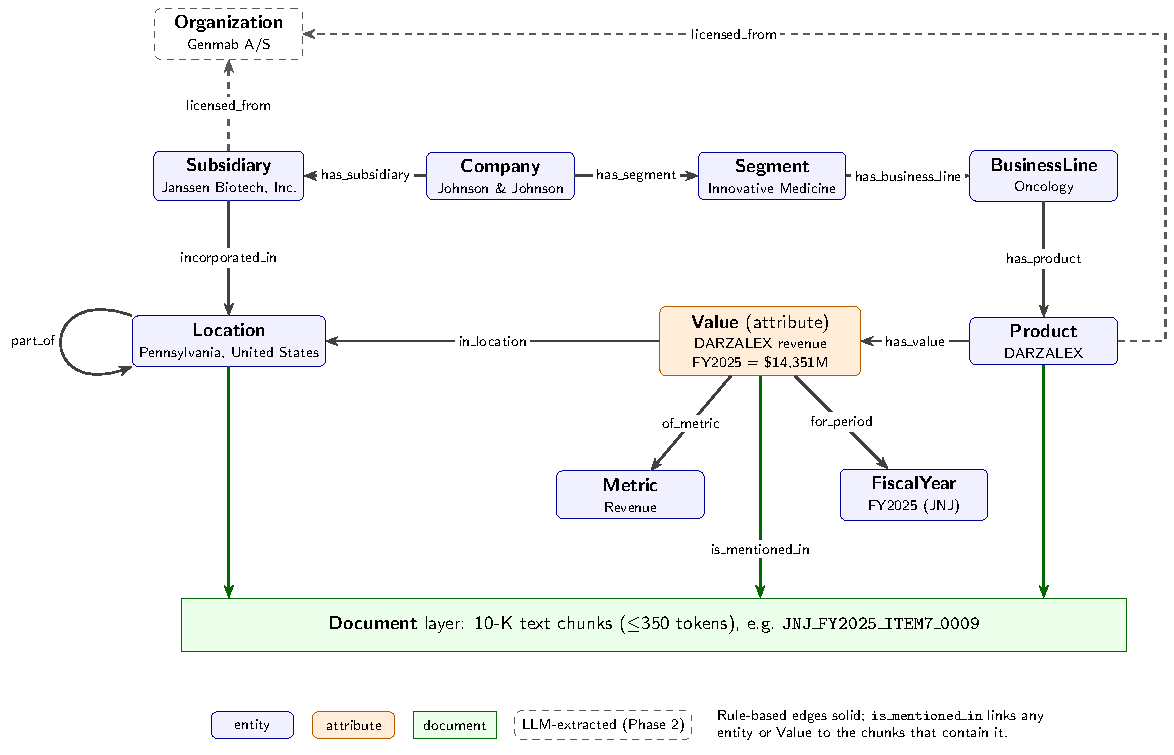
\includegraphics[width=0.92\textwidth]{schema_figure.pdf}
  \caption{Graph schema, shown with the nodes of our multi-hop seed question. Rule-based edges
  (solid) come from Exhibit~21 and the inline XBRL tags; dashed edges are extracted from the text by
  an LLM (Phase~2, in progress). \texttt{is\_mentioned\_in} connects any entity or Value to the
  document chunks that contain it.}
  \label{fig:schema}
\end{figure*}

\subsection{Graph construction}
\label{sec:construction}
For this report the graph covers three of the eight companies (Johnson \& Johnson, Apple and
Microsoft; six filings), which overlap most with our golden questions and include the seed example.
Construction has two phases.

\paragraph{Phase 1: rules over structured sources.}
Subsidiaries and jurisdictions are read from the Exhibit~21 tables; jurisdictions are normalized
(\eg ``Delaware, U.S.''~$\rightarrow$ Delaware) and U.S.\ states are linked to the United States by
\texttt{part\_of}. Segments, business lines, products, regions and numbers come from the inline XBRL
tags. We keep 26 common concepts (revenue, cost of sales, R\&D expense, operating and net income,
earnings per share, total assets, operating cash flow and others), only full fiscal-year periods or
year-end balances, and only facts whose dimensions are segment, sub-segment, product or geography.
The dimensions of a fact give the hierarchy: a revenue fact tagged with Innovative Medicine, Oncology
and DARZALEX yields Company $\rightarrow$ Segment $\rightarrow$ BusinessLine $\rightarrow$ Product.
A fact that appears in both filings of a company is stored once, with the newer value.
\texttt{is\_mentioned\_in} edges come from whole-word name matching within the same company's
chunks; a Value is linked to a chunk only if the chunk prints the same number and names its subject
or metric. The files follow gfmrag's ``bring your own graph'' format and pass a validation script
that reads them the way the loader does. \Cref{tab:graph} summarizes the result, \texttt{fin10k\_v0}.

\begin{table*}[t]
  \centering
  \resizebox{\textwidth}{!}{%
  \begin{tabular}{llr rrr rrr}
    \toprule
    & & & \multicolumn{3}{c}{Nodes by type} & \multicolumn{3}{c}{Edges by type} \\
    \cmidrule(lr){4-6}\cmidrule(lr){7-9}
    Company & Filings (fiscal year) & Chunks & Entity & Attribute & Document & Structural & Value & Mention \\
    \midrule
    Johnson \& Johnson & FY2024, FY2025 & 440 + 433 & 480 & 726 & 873 & 903 & 2,590 & 6,000 \\
    Apple              & FY2024, FY2025 & 194 + 198 &  37 & 176 & 392 &  51 &   540 & 1,600 \\
    Microsoft          & FY2025, FY2026 & 290 + 300 &  30 & 192 & 590 &  33 &   584 & 2,111 \\
    Shared (locations, metrics) & --    & --        & 122 & --  & --  &  19 &    -- &    -- \\
    \midrule
    Total              & 6 filings      & 1,855     & 669 & 1,094 & 1,855 & 1,006 & 3,714 & 9,711 \\
    \bottomrule
  \end{tabular}}
  \caption{The rule-based graph \texttt{fin10k\_v0}. Chunks are listed per filing in fiscal-year
  order. Entity nodes: 3 companies, 450 subsidiaries, 101 locations, 11 segments, 10 business lines,
  60 products, 21 metrics, 13 fiscal years. Structural edges: \texttt{has\_subsidiary},
  \texttt{incorporated\_in}, \texttt{part\_of}, \texttt{has\_segment}, \texttt{has\_business\_line},
  \texttt{has\_product}; Value edges: \texttt{has\_value}, \texttt{of\_metric}, \texttt{for\_period},
  \texttt{in\_location}; Mention edges: \texttt{is\_mentioned\_in}. The full eight-company corpus has
  7,339 chunks.}
  \label{tab:graph}
\end{table*}

\paragraph{Phase 2: relations written in prose (in progress).}
Some relations appear only in sentences, such as the DARZALEX license from Genmab. We prompt Gemini
(\texttt{gemini-3.5-flash-lite}) on the 623 text chunks of Items~1, 7 and~8 of the same six filings to
return triples of nine types (\texttt{licensed\_from}, \texttt{acquired}, \texttt{partners\_with},
\texttt{competes\_with}, \texttt{manufactures}, \texttt{supplies\_to}, \texttt{has\_product},
\texttt{subsidiary\_of}, \texttt{invests\_in}), each with a supporting quote. A triple is kept only
if its quote appears in the chunk and both names are specific; names are then merged into existing
nodes. All 623 chunks have been processed, giving 1,026 candidate triples from 272 chunks (78\% of
them \texttt{has\_product}); filtering, merging into the graph (\texttt{fin10k\_v1}) and a hand
check are still to be done. On a five-chunk pilot the extractor recovered the full DARZALEX chain
(Janssen Biotech \texttt{licensed\_from} Genmab~A/S).

\subsection{Query-conditioned graph retriever}
\label{sec:retriever}
Given a question $q$, entity linking selects a set of start nodes $S_q$ in the graph. A
query-dependent GNN then propagates information from $S_q$ along typed edges. Schematically, with
$\mathbf{e}_q$ the question embedding, $\mathbf{x}_v$ the text embedding of node $v$ and
$\mathcal{N}(v)$ its in-neighbors with relations $r$,
\begin{align}
  \mathbf{h}_v^{(0)} &= \mathbb{1}[v \in S_q]\,\mathbf{e}_q, \label{eq:init}\\
  \mathbf{h}_v^{(\ell+1)} &= \phi\Big(\mathbf{h}_v^{(\ell)},\;
     \textstyle\bigoplus_{(u,r)\in\mathcal{N}(v)} \psi\big(\mathbf{h}_u^{(\ell)}, \mathbf{x}_u,
     \mathbf{e}_r, \mathbf{e}_q\big)\Big), \label{eq:mp}\\
  s(v \mid q) &= \sigma\big(\mathrm{MLP}(\mathbf{h}_v^{(L)})\big), \label{eq:score}
\end{align}
where $\psi$ builds a message, $\bigoplus$ aggregates messages and $\phi$ updates the node state. The
top-$k$ document nodes by $s(v\mid q)$ are the retrieved chunks. We use the pretrained
\texttt{G-reasoner-34M} checkpoint~\cite{luo2026greasoner} through the gfmrag library, with node and
relation text embedded by Qwen3-Embedding-0.6B. Start nodes come from a rule-based matcher that maps
names and aliases in the question to graph entities (\eg ``Apple'' $\rightarrow$ Apple Inc.,
``fiscal 2025'' $\rightarrow$ FY2025 (AAPL), ``net sales'' $\rightarrow$ Revenue).

\paragraph{Fine-tuning (next).}
Following G-reasoner's training recipe, fine-tuning combines a supervised loss on the target nodes
$T_q$ of each training question (written here as binary cross-entropy) with a distillation term that keeps the model close to the
relevance distribution $p_{\text{dense}}$ of a frozen text-embedding model:
\begin{multline}
  \mathcal{L} = -\sum_{v} \Big[y_v \log s(v\mid q) + (1-y_v)\log\big(1-s(v\mid q)\big)\Big]\\
  + \lambda\, \mathrm{KL}\big(p_{\text{dense}}(\cdot\mid q)\,\|\,p_\theta(\cdot\mid q)\big),
  \label{eq:loss}
\end{multline}
with $y_v = \mathbb{1}[v\in T_q]$. Training pairs are generated from graph paths with six templates
(\cref{tab:synthetic}). Every pair records its start nodes, target nodes, gold path and computed
answer. Microsoft is held out for testing, and 51 pairs that ask for a number appearing in a
golden-set answer are excluded from both splits so the golden questions stay unseen.

\begin{table}[t]
  \centering
  \footnotesize
  \setlength{\tabcolsep}{4pt}
  \begin{tabular}{@{}llr@{}}
    \toprule
    Template & Gold path & Pairs \\
    \midrule
    lookup     & subject $\rightarrow$ Value $\rightarrow$ chunk & 600 \\
    change     & one subject and metric, two years & 600 \\
    hierarchy  & segment $\rightarrow$ product $\rightarrow$ Value & 123 \\
    share      & product / company revenue & 219 \\
    compare    & one metric, two companies & 147 \\
    subsidiary & company $\rightarrow$ subsidiary $\rightarrow$ place & 446 \\
    \midrule
    \multicolumn{2}{@{}l}{Train (J\&J, Apple)} & 1,734 \\
    \multicolumn{2}{@{}l}{Test (Microsoft held out)} & 350 \\
    \multicolumn{2}{@{}l}{Excluded (overlap with golden answers)} & 51 \\
    \bottomrule
  \end{tabular}
  \caption{Synthetic question--subgraph pairs generated from \texttt{fin10k\_v0} for fine-tuning.}
  \label{tab:synthetic}
\end{table}

\paragraph{LLM interface (planned).}
The retrieved nodes and the edges between them will be pruned to a compact connected subgraph and
passed, with their source chunks, to an LLM that answers the question and cites the nodes and edges
it used, following the G-Retriever design~\cite{he2024gretriever}.

% =====================================================================================
\section{Experiments and Results}
\label{sec:experiments}

\subsection{Setup}
\label{sec:setup}
\paragraph{Golden set.}
The golden set has 19 questions over the eight companies: 9 single-fact, 5 multi-hop within one
company and 5 comparing two companies. Each has gold chunk IDs and a gold answer. Gold chunks came
from pattern matching (a label plus a number, \eg ``Total net sales $|$ \$416,161''); an independent
LLM labeling pass with quote verification has so far validated one question (q01), so all numbers
below are preliminary. Eleven questions fall on the three companies in \texttt{fin10k\_v0} and are
used to compare against the graph retriever.

\paragraph{Metrics.}
For a question with gold chunks $G$ and ranked retrieved list $R$, with $R_k$ its top $k$,
\begin{equation}
  \begin{gathered}
  \mathrm{P@}k = \frac{|R_k \cap G|}{k},\qquad
  \mathrm{R@}k = \frac{|R_k \cap G|}{|G|},\\
  \mathrm{Hit@}k = \mathbb{1}\big[\,|R_k \cap G| > 0\,\big],
  \end{gathered}
  \label{eq:metrics}
\end{equation}
averaged over questions, with $k\in\{5,10\}$. Answers are judged by an LLM (Gemini~2.5 Flash) as
correct, hallucinated (a wrong figure or fact) or missing (no answer), and we record retrieval and
end-to-end latency.

\paragraph{Systems.}
The vector baselines embed chunks with \texttt{bge-small-en-v1.5}~\cite{xiao2023cpack} (33M) or a
DistilBERT bi-encoder (66M), search a FAISS inner-product index over L2-normalized vectors, and
optionally rerank the top 20 with the cross-encoder \texttt{ms-marco-MiniLM-L-6-v2}; answers are
generated by Gemini~2.5 Flash-Lite at temperature~0. G-reasoner runs on a Colab T4 GPU.

\subsection{Vector-RAG baseline}
\label{sec:exp-baseline}
\Cref{tab:baseline} shows the baseline on all 19 questions. bge-small finds a gold chunk in the top
10 for 79\% of questions, but only 42--47\% of answers are judged correct. Reranking raises recall at
$k{=}10$ and lowers the share of missing answers, but also raises the hallucination rate. The errors
are informative for our project: retrieval never picks the wrong company, but picks the wrong fiscal
year of the right company in 43\% of cases, and cross-company questions almost never retrieve the
answer chunks of both companies. Generation takes about 94\% of the end-to-end time.

\begin{table}[t]
  \centering
  \footnotesize
  \setlength{\tabcolsep}{3pt}
  \begin{tabular}{@{}lc ccc ccc@{}}
    \toprule
    Config & $k$ & P@$k$ & R@$k$ & Hit@$k$ & Corr. & Hall. & Miss. \\
    \midrule
    bge-small          & 5  & .19 & .39 & .74 & .42 & .05 & .53 \\
    bge-small          & 10 & .13 & .50 & .79 & .47 & .11 & .42 \\
    bge-small+rerank & 5  & .19 & .37 & .68 & .47 & .21 & .32 \\
    bge-small+rerank & 10 & .13 & .51 & .84 & .47 & .21 & .32 \\
    DistilBERT         & 5  & .16 & .32 & .63 & .32 & .05 & .63 \\
    DistilBERT         & 10 & .12 & .41 & .68 & .37 & .11 & .53 \\
    \bottomrule
  \end{tabular}
  \caption{Vector-RAG baseline on the 19 golden questions (preliminary labels). Corr./Hall./Miss.\
  are the shares of answers judged correct, hallucinated or missing. Retrieval takes about 13\,ms
  (50\,ms with reranking); end-to-end about 0.5\,s per question.}
  \label{tab:baseline}
\end{table}

\subsection{Zero-shot G-reasoner}
\label{sec:exp-greasoner}
\Cref{tab:greasoner} compares retrievers on the 11 golden questions covered by the graph.
Zero-shot G-reasoner finds a gold chunk for only 2 of 11 questions (Hit@5 0.18), against 0.91 for
bge-small. Ranking the document nodes by cosine similarity between the question and G-reasoner's own node
features (Qwen3 embeddings) reaches 0.82, so the graph and its text features carry the needed
information; the loss comes from the pretrained GNN's ranking. Inspecting the outputs, G-reasoner
starts from the right company and fiscal year but ranks generic chunks of that filing first (for
example, three of its top five chunks for a question about Apple's net sales are risk-factor or
business-overview passages).

\begin{table}[t]
  \centering
  \footnotesize
  \setlength{\tabcolsep}{4pt}
  \begin{tabular}{@{}lcccc@{}}
    \toprule
    System & Hit@5 & R@5 & Hit@10 & R@10 \\
    \midrule
    Vector RAG, bge-small        & 0.91 & 0.41 & 1.00 & 0.56 \\
    Vector RAG, + rerank         & 0.82 & 0.42 & 0.91 & 0.60 \\
    Dense on graph node features & 0.82 & 0.60 & 0.91 & 0.76 \\
    \textbf{G-reasoner, zero-shot} & \textbf{0.18} & \textbf{0.04} & \textbf{0.18} & \textbf{0.04} \\
    G-reasoner, fine-tuned           & \multicolumn{4}{c}{\emph{planned}} \\
    LightRAG / HippoRAG 2            & \multicolumn{4}{c}{\emph{planned}} \\
    \bottomrule
  \end{tabular}
  \caption{Document retrieval on the 11 golden questions covered by \texttt{fin10k\_v0}. With 11
  questions, one question changes Hit@$k$ by 0.09.}
  \label{tab:greasoner}
\end{table}

\subsection{Diagnosis and ablation}
\label{sec:exp-ablation}
\paragraph{Hub start nodes.}
Company and FiscalYear nodes are linked to every chunk of their filing through the chunk header, so
they act as hubs. Removing them from the start nodes does not help (Hit@5 0.00, Hit@10 0.09), and
using only them gives 0.00, so the hubs are needed to find the right filing but do not, on their own,
explain the poor ranking.

\paragraph{Rule-based vs.\ LLM start nodes.}
gfmrag's default chooses start nodes with an LLM. Letting Gemini (\texttt{gemini-3.5-flash-lite})
choose them from the 669 entity names gave the same start nodes as our rule-based matcher on all
11 questions and identical retrieved lists, while adding about 1.3\,s per question (matching plus
retrieval about 1.41\,s vs.\ 0.11\,s). On nine paraphrased probe questions each method was better on
two. We keep the rule-based matcher, which is faster and deterministic.

\subsection{Graph quality and known issues}
\label{sec:exp-issues}
We checked 30 randomly sampled edges of \texttt{fin10k\_v0} against the filings and found 29
correct (97\%); the one error was a place name matched inside a court name (``United States
District Court''). Two weaker patterns were mentions inside legal notes and products linked to the
company rather than their segment. Beyond this sample, we found the following problems, which we
will fix before the final experiments:
\begin{itemize}
  \item \textbf{J\&J R\&D values are wrong.} J\&J tags two R\&D concepts in XBRL: total R\&D
  (excluding acquired in-process R\&D) and the acquired in-process R\&D charges alone. Our build
  maps both to one metric and the second overwrote the first, so the graph gives \$109M for FY2025 instead of \$14,665M. This affects
  golden questions q06, q14 and q18 and was excluded from the synthetic data.
  \item \textbf{Coverage.} The graph has 3 of 8 companies, so 8 of 19 golden questions cannot yet be
  scored for the graph retriever.
  \item \textbf{Golden set.} Only 1 of 19 gold labels is validated, and the multi-hop questions
  are mostly arithmetic or two-company comparisons; none yet follows a relation chain such as
  subsidiary $\rightarrow$ license $\rightarrow$ product, which is where a graph retriever should help.
  \item \textbf{Entity matcher.} On paraphrases, the rule-based matcher maps ``sales and marketing''
  to Revenue and ``operating profit'' to Net income, and does not resolve relative dates
  (``last year'').
  \item \textbf{Model versions.} The baseline generates answers with Gemini~2.5 Flash-Lite, which
  new API keys can no longer use, so one generator must be agreed on before comparing answers.
  \item \textbf{Value nodes.} G-reasoner's top-ranked Value nodes barely depend on the question, so
  retrieved numbers are not used as evidence until after fine-tuning.
\end{itemize}

% =====================================================================================
\section{Conclusions}
\label{sec:conclusions}
The data pipeline, the graph and both retrievers now run end to end. Three findings shape the rest
of the project. First, a graph built only from structured parts of a 10-K, the subsidiary exhibit
and the XBRL tags, is accurate (29 of 30 checked edges) and already supports the relation chains in
our seed question, but structured sources hide their own traps, as the two J\&J R\&D concepts
show. Second, a pretrained graph retriever does not transfer to this domain zero-shot: it reaches the
right filing but not the right passage, even though dense search over the same node features
works. Fine-tuning is therefore the central experiment, not an optional improvement. Third, the
evaluation needs as much work as the models: the golden set must be validated and extended with
relation-chain questions before any difference between retrievers can be trusted.
Next, we will fix the R\&D mapping, add the LLM-extracted relations and the other five companies,
validate and extend the golden set, fine-tune G-reasoner on the synthetic pairs, and build the
subgraph-to-LLM interface, then compare against vector RAG, reranking, LightRAG and HippoRAG~2 with
ablations on the loss and the graph construction.

\paragraph{Code.} \url{https://github.com/memnaaaaa/financial-graphrag} (data pipeline, graph
construction, baselines, G-reasoner scripts and results).

% =====================================================================================
\clearpage
\section*{Peer Evaluation}
Mohini Tiwari collected the filings, built the chunk corpus and the knowledge graph (schema, rule-based
construction, LLM relation extraction, hand check) and wrote the Related Work and the filings and
schema parts of the Method. Mahua Mahua built the vector-RAG baselines, the golden question set, the
evaluation metrics and the LLM judge. Rida Hameed Syeda set up and ran G-reasoner on our graph,
diagnosed its zero-shot results, ran the start-node ablation and built the synthetic question
generator. All three of us contributed to the report.

\begin{table}[h]
  \centering
  \small
  \begin{tabular}{|l|c|}
    \hline
    Mahua Mahua & \underline{\hspace{2em}} / 20 \\
    Rida Hameed Syeda & \underline{\hspace{2em}} / 20 \\
    Myself (Mohini Tiwari) & \underline{\hspace{2em}} / 20 \\
    \hline
  \end{tabular}
  \caption{Self-peer evaluation (scores to be completed for the final report).}
  \label{tab:peer}
\end{table}

{
  \small
  \bibliographystyle{ieeenat_fullname}
  \bibliography{refs}
}

\end{document}
